\chapter{Анализ случайных графов и оценка расстояний между структурами}
\label{chap:random_graphs}

\section{Математическое ожидание числа компонент заданного размера}

Одним из важнейших параметров рассматриваемой модели является количество компонент (связных частей графа) заданного размера. Для ясности сначала рассмотрим случаи небольшого размера (например, компоненты из одного элемента), а затем получим общую формулу для произвольного размера $m$. Наконец, будет обсуждена асимптотика появления ``гигантской'' компоненты при увеличении размера.

\subsection{Компоненты размера 1}

Рассмотрим вероятность того, что определённая связь (ребро) остаётся неизменной после случайных преобразований. Пусть всего имеется $n$ элементов (блоков) и соответственно $n$ возможных связей между ними. Каждая связь $i$ (адресованная соответствующим параллельным фрагментам в двух структурах) характеризуется показателем ``хрупкости'' $p_i \in [0,1]$, отражающим вероятность участия этой связи в случайной перестройке на каждом шаге. Предполагается, что значения $p_i$ нормированы и суммарно образуют распределение вероятностей на множестве связей: $\sum_{i=1}^n p_i = 1$. На каждом элементарном шаге происходит случайное преобразование структуры, в ходе которого выбираются две связи (не обязательно различные, если операция разрыва-вставки затрагивает одну связь дважды) для перестройки. Таким образом, на каждом шаге вероятность того, что именно $i$-я связь будет вовлечена в операцию, равна $2 p_i$. 

Пусть за всю историю произошло $k$ случайных операций. Тогда вероятность того, что фиксированное $i$-е ребро \emph{никогда} не участвовало ни в одной из $k$ перестроек, равна $(1 - p_i)^{2k}$ (так как на каждом из $k$ шагов данная связь должна остаться вне двух задействованных связей). Введём индикаторную случайную величину 
$$\mathbf{1}_{\{\text{$i$-я связь не затронута}\}},$$
которая равна 1, если связь $i$ осталась нетронутой, и 0 иначе. Общее число компонент размера 1 (то есть отдельных связей, сохранившихся неизменными) обозначим $c_1 = \sum_{i=1}^n \mathbf{1}_{\{\text{$i$-я связь не затронута}\}}$. Тогда по определению математического ожидания
\[
E(c_1) \;=\; \sum_{i=1}^n P(\text{$i$-я связь не участвовала в перестройках}) \;=\; \sum_{i=1}^n (1 - p_i)^{2k} \,. 
\]
Нас будет интересовать нормированное значение, то есть средняя доля таких связей:
\[
E\!\Big(\frac{c_1}{n}\Big) \;=\; \frac{1}{n} \sum_{i=1}^n (1 - p_i)^{2k} \,.
\]
Для дальнейшего анализа будем считать число элементов $n$ большим и перейти к предельному случаю $n \to \infty$. Одновременно будем полагать, что число операций $k$ линейно зависит от $n$. А именно, предположим, что существует постоянная $\gamma > 0$ такая, что 
\[
\frac{2k}{n} \;\to\; \gamma \quad \text{при } n \to \infty\,,
\] 
то есть $k \sim \frac{\gamma n}{2}$. Таким образом, $\gamma$ характеризует \emph{интенсивность} перестроек (ожидаемое число операций на элемент структуры).

Заметим, что при указанных предположениях величины $p_i$ сами по себе случайны и, вообще говоря, различны для разных $i$. В модели предполагается, что значения $p_i$ независимы и одинаково распределены: интенсивности ``хрупкости'' фрагментов подчиняются некоторому распределению. Мы будем рассматривать \emph{равномерный случай}, когда показатели $p_i$ имеют так называемое ``плоское'' распределение Дирихле, соответствующее отсутствию априорных предпочтений (все фрагменты структуры в среднем одинаково хрупки). В этом случае можно считать, что случайные величины $\alpha_i = n p_i$ являются независимыми экспоненциальными величинами с единичным математическим ожиданием. Иными словами, при $n \to \infty$ суммарная мера $M = \sum_{i=1}^n \alpha_i$ по закону больших чисел будет близка к $n$ (более строго, $\frac{M}{n} \to 1$ при $n \to \infty$). Это даёт приближение $p_i = \frac{\alpha_i}{M} \approx \frac{\alpha_i}{n}$ для каждого $i$. Используя это и предположение о линейном росте $k$, можем оценить:
\[
(1 - p_i)^{2k} \;=\; \Big(1 - \frac{\alpha_i}{M}\Big)^{2k} \;\approx\; \Big(1 - \frac{\alpha_i}{n}\Big)^{\gamma n} \;\xrightarrow[n \to \infty]{}\; e^{-\gamma \alpha_i}\,,
\] 
поскольку $\frac{M}{n} \to 1$. Таким образом, 
\[
E\!\Big(\frac{c_1}{n}\Big) \;\approx\; \frac{1}{n}\sum_{i=1}^n e^{-\gamma \alpha_i}\,. 
\]
Так как $\alpha_i$ независимы и распределены по экспоненциальному закону с плотностью $f(\alpha) = e^{-\alpha}$ на $\R_+,$ то можно проинтегрировать полученное выражение по распределению $\alpha_i$. Практически это означает, что при больших $n$ сумма $\frac{1}{n}\sum_{i} e^{-\gamma \alpha_i}$ близка к математическому ожиданию $E(e^{-\gamma \alpha})$ для одной экспоненциальной величины $\alpha$. Последнее легко находится напрямую:
\[
E(e^{-\gamma \alpha}) \;=\; \int_{0}^{\infty} e^{-\gamma \alpha} e^{-\alpha} d\alpha \;=\; \int_{0}^{\infty} e^{-(\gamma+1)\alpha}\, d\alpha \;=\; \frac{1}{\gamma+1}\,.
\] 
Отсюда получаем предельную долю неизменных связей:
\[
\lim_{n \to \infty} E\!\Big(\frac{c_1}{n}\Big) \;=\; \frac{1}{\,1 + \gamma\,}\,.
\] 
Другими словами, при большом количестве элементов $n$ и фиксированном отношении $\gamma = 2k/n$, в среднем доля компонент размером 1 равна $\frac{1}{1+\gamma}$. Например, если число операций $k$ примерно равно числу элементов ($\gamma \approx 2$), то лишь порядка $1/(1+2) \approx 33\%$ связей остаются нетронутыми; если же операций существенно меньше ($\gamma \ll 1$), то значительная часть ($\approx 100\%$ при $\gamma \to 0$) исходных связей сохранится.

Аналогичным образом можно получить выражение для числа компонент, состоящих из двух элементов. В контексте задачи такие компоненты размера $2$ соответствуют появлению цикла длины 2 (пары связанных элементов) в результирующей структуре. Пусть фиксированы два конкретных ребра (связи) $i$ и $j$. Для того чтобы из них образовалась отдельная компонента (цикл длины 2), необходимо, чтобы на одном из шагов эти связи были одновременно выбраны для перестройки и при этом склеены вместе, а на всех остальных шагах ни $i$, ни $j$ не участвовали в операциях. Вероятность того, что на некотором заданном шаге выбраны именно $i$ и $j$, приблизительно равна $p_i p_j$ (для простоты принимая независимость выборов, поскольку $p_i, p_j \ll 1$ при большом $n$). Поскольку подходящий шаг может быть любым из $k$, суммарная вероятность того, что \emph{существует} шаг, на котором произошла перестройка с участием именно этих двух связей, оценится как $k\,p_i p_j$. Зафиксировав такой шаг, требуется, чтобы на всех остальных $(k-1)$ шагах связи $i$ и $j$ не затрагивались; вероятность этого равна $(1 - p_i - p_j)^{2(k-1)}$ (на каждом из остальных шагов ни одна из двух связей не должна попасть в выбранную пару). Перемножая указанные факторы, получаем вероятность конкретного сценария образования компоненты $\{i,j\}$: 
\[ 
P(\text{связи $i,j$ образуют цикл длины $2$}) \;\approx\; k\, p_i\, p_j\, \big(1 - p_i - p_j\big)^{2(k-1)}\,.
\] 
Просуммировав эту вероятность по всем упорядоченным парам $(i,j)$ (где $1 \le i < j \le n$), получим математическое ожидание общего числа таких компонентов. Нормируя на $n$, запишем:
\[
E\!\Big(\frac{c_2}{n}\Big) \;=\; \frac{1}{n} \sum_{1 \le i < j \le n} k\, p_i\, p_j\, \big(1 - p_i - p_j\big)^{2(k-1)}\,.
\]
Далее, аналогично случаю $m=1$, можно провести предельный переход $n \to \infty$. При больших $n$ и $\gamma = 2k/n = \text{const}$ величины $p_i$ малые, и вышеуказанная сумма может быть проинтегрирована, заменив $p_i = \alpha_i/n$, $p_j = \alpha_j/n$ и используя экспоненциальное распределение $\alpha_i$. В результате получается некоторое явное выражение в замкнутом виде через $\gamma$. Тем не менее, вместо того чтобы отдельно вычислять частные случаи $m=1,2$, целесообразно сразу приступить к выводу общей формулы для компоненты произвольного размера $m$. При этом перечисленные частные случаи (для $m=1$ и $m=2$) будут получены как следствия общей формулы.

\subsection{Компоненты произвольного размера}

Теперь рассмотрим произвольное фиксированное число $m \ge 1$ и вычислим математическое ожидание $E(c_m)$, где $c_m$ -- случайное число компонент (в результирующей структуре) размера $m$. В терминах графовой модели это означает, что нас интересует число циклов длины $m$, образовавшихся после $k$ случайных перестроек. Для простоты дальнейшего изложения будем называть базовые прочные фрагменты структуры \emph{блоками}. Тогда цикл длины $m$ соответствует объединению $m$ различных блоков в одну компоненту.

Рассмотрим некоторое фиксированное подмножество из $m$ определённых блоков (скажем, блоки с номерами $1,2,\dots,m$) и исследуем вероятность того, что именно эти $m$ блоков в итоге образуют единый цикл (компоненту размера $m$). Очевидно, что для образования цикла из $m$ блоков необходимо совершить ровно $m-1$ операций, каждая из которых соединяет между собой две разрозненные группы блоков. Поскольку всего совершается $k$ операций, то нам нужно сначала выбрать, на каких шагах происходили эти $m-1$ объединений. Число способов выбрать $m-1$ шагов из $k$ равно $\binom{k}{\,m-1\,}$. Далее, когда выбраны шаги, необходимо определить, каким образом на этих шагах происходило слияние указанных $m$ блоков в единый цикл. Этот процесс можно описать последовательностью упорядоченных пар $(i,j)$, где $i$ и $j$ -- номера блоков, которые объединяются на данном шаге (причём договариваемся всегда указывать $i<j$). Такая последовательность пар кодирует \emph{сценарий} объединения блоков. Например, на рис.~\ref{merge-into-cycle} показан сценарий объединения 4 блоков с номерами $1,2,3,4$ в цикл длины 4, задаваемый последовательностью $a_{13},\,a_{23},\,a_{34}$ (здесь $a_{ij}$ обозначает операцию слияния блоков $i$ и $j$ на соответствующем шаге). 

\begin{figure}[h!]
    \centering
    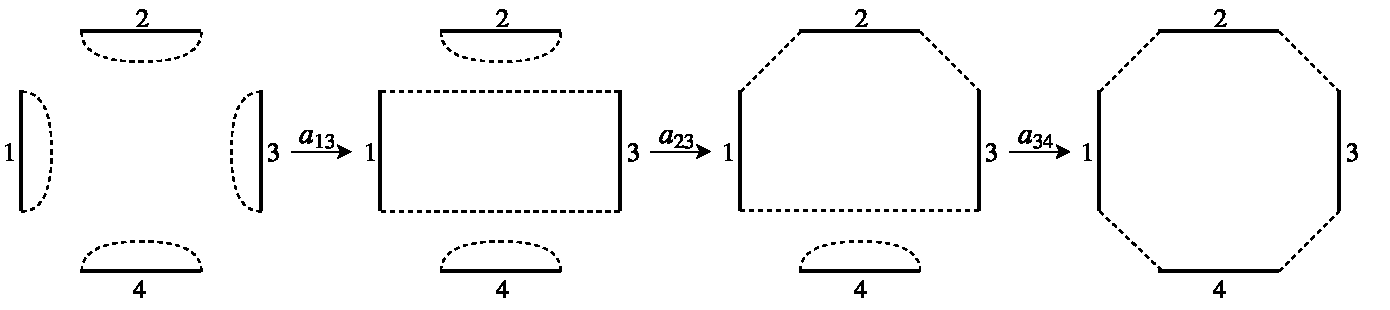
\includegraphics[width=\linewidth]{images/part2/merge-into-cycle.pdf}
    \caption{Пример объединения в цикл длины $4$ (сценарий: $a_{13},\,a_{23},\,a_{34}$).}
    \label{merge-into-cycle}
\end{figure}

При такой визуализации блоки пронумерованы для наглядности, но следует иметь в виду, что эти номера соответствуют определённым исходным связям (потенциальным разрывам) между блоками. Иными словами, операции происходят над связями, соединяющими блоки в исходной конфигурации: когда говорится, что выполняется операция $a_{ij}$, подразумевается, что на данном шаге выбраны связи, инцидентные блокам $i$ и $j$ (каждый блок соединён в исходной структуре двумя связями с соседями, если рассматривать структуру как граф). Таким образом, слияние блоков $i$ и $j$ в рамках одной операции означает, что разрываются связи, ранее соединявшие эти блоки с их соседями, и затем блок $i$ и $j$ становятся соседними в новой структуре (образуя часть цикла).

Каждый сценарий объединения $m$ фиксированных блоков в цикл можно однозначно отобразить на помеченное дерево с $m$ вершинами (так называемое остовное дерево, соединяющее эти $m$ элементов).
Блоки $1,2,\dots,m$ станут вершинами такого дерева. Проведём ребро между вершинами $i$ и $j$ в дереве, если в сценарии имеется шаг $a_{ij}$ (то есть на одном из шагов были объединены блоки $i$ и $j$).
На рис.~\ref{tree-bijection} представлен пример остовного дерева, соответствующего приведённому выше сценарию (для блоков $1,2,3,4$).
Легко видеть, что построенное соответствие является биекцией: каждому возможному сценарию объединения $m$ блоков соответствует единственное дерево на этих $m$ вершинах, и наоборот, любое остовное дерево на $m$ узлах задаёт ровно один сценарий слияния блоков.
Однако эта биекция не является однозначной, а имеет определённый коэффициент кратности. Действительно, дерево не отражает порядка, в котором производились операции (то есть все $m-1$ шагов могут идти в разном хронологическом порядке, приводя к одному и тому же конечному результату).
Перестановок $m-1$ шагов существует $(m-1)!$ штук, что даёт соответствующий множитель. Кроме того, каждая отдельная операция слияния могла происходить в одном из двух ``направлений'', то есть при заданных двух выбранных связях есть два варианта, как именно соединить их концами при перестройке (обе возможности приводят к объединению циклов, но различаются переставляемыми концами разорванных связей).
Для цикла произвольной длины каждый из $m-1$ шагов обладает двумя такими вариантами, что даёт множитель $2^{\,m-1}$. Таким образом, одному остовному дереву соответствует $2^{\,m-1}(m-1)!$ различных сценариев слияния. 

\begin{figure}[h!]
    \centering
    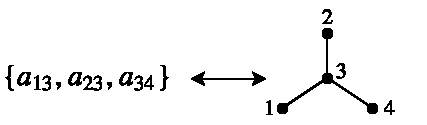
\includegraphics[width=3in]{images/part2/tree-bijection.pdf}
    \caption{Пример биекции сценария с остовным деревом для $m=4$.}
    \label{tree-bijection}
\end{figure}

Теперь оценим суммарную вероятность всех возможных сценариев, приводящих к объединению заданных блоков $1,\dots,m$ в один цикл.
Как отмечалось выше, на определённом шаге операция затрагивает связи, инцидентные некоторым блокам.
Предположим, что показатель хрупкости каждого из выбранных $m$ блоков оставался постоянным на всём протяжении процесса и равен $p_i$ для $i$-го блока.
Тогда вероятность конкретного сценария $S$ можно разложить по шагам: на каждом шаге, когда объединяются блоки $i$ и $j$, в вероятность входит множитель $p_i p_j$ (пропорционально вероятности выбора связей этих блоков).
Таким образом, вероятность сценария $S$ равна произведению $p_i^{\,d_i}$ по всем $i$ из $\{1,\dots,m\}$, где $d_i$ -- степень вершины $i$ в соответствующем дереве $T_S$.
Иными словами, $d_i$ равно числу операций, в которых участвовал $i$-й блок при данном сценарии.
Поэтому вероятность сценария $S$ запишется как 

\[
P(S) \;=\; \prod_{i=1}^{m} p_i^{\,d_i}\,. 
\] 
Чтобы найти искомую суммарную вероятность, нужно просуммировать $P(S)$ по всем сценариям $S$, приводящим к объединению блоков $1,\dots,m$. Благодаря описанной выше биекции, вместо суммирования по сценариям можно суммировать по всем возможным помеченным деревьям $T$ на $m$ вершинах, учитывая множитель кратности $2^{\,m-1}(m-1)!$ сценариев на одно дерево. То есть 
\[
\sum_{S} P(S) \;=\; 2^{\,m-1}(m-1)!\, \sum_{T} \prod_{i=1}^m p_i^{\,d_i(T)}\,,
\] 
где сумма справа берётся по всем остовным деревьям $T$, соединяющим вершины $1,\dots,m$, а $d_i(T)$ -- степень вершины $i$ в дереве $T$. Известный результат комбинаторики (следствие кодировки Прюфера для labeled-деревьев) гласит, что 
\[
\sum_{T} \prod_{i=1}^m p_i^{\,d_i(T)} \;=\; (p_1 + p_2 + \cdots + p_m)^{\,m-2}\, p_1 p_2 \cdots p_m\,.
\] 
Действительно, число различных помеченных деревьев на $m$ заданных вершинах равно $m^{\,m-2}$ (формула Кэли), а указанное взвешенное суммирование приводит именно к указанной комбинации (её можно вывести напрямую из представления дерева кодом Прюфера длины $m-2$). Таким образом, мы получили значение суммарной вероятности:
\[
\sum_{S} P(S) \;=\; 2^{\,m-1}(m-1)!\, p_1 p_2 \cdots p_m\, (p_1 + p_2 + \cdots + p_m)^{\,m-2}\,. 
\]
Именно эта величина и представляет собой вероятность того, что выбранные блоки $1,\dots,m$ объединятся в единый цикл длины $m$ (через все возможные сценарии). Формально данный результат можно сформулировать в виде леммы.

\begin{lemma}\label{lem:prufer}
Для фиксированного набора из $m$ блоков с показателями хрупкости $p_1, p_2, \dots, p_m$ суммарная вероятность всех сценариев, приводящих к слиянию этих блоков в одну компоненту (цикл) размера $m$, равна
\[
2^{\,m-1}(m-1)!\; p_1 p_2 \cdots p_m \; (p_1 + p_2 + \cdots + p_m)^{\,m-2}\,.
\] 
\end{lemma}

Итак, для фиксированных $m$ блоков мы вывели вероятность того, что они образуют цикл длины $m$ в результате $k$ перестроек. Теперь получим выражение для математического ожидания общего числа таких компонент $c_m$. Заметим, что различных наборов из $m$ блоков (которые могут образовать компоненту) всего $\binom{n}{m}$. Вероятность для каждого из них определяется формулой из леммы~\ref{lem:prufer} выше. При суммировании по всем комбинациям нужно также учесть, что указанные события (образования конкретных циклов) не являются независимыми; однако при вычислении \emph{математического ожидания} мы можем воспользоваться принципом линейности ожидания и просуммировать вероятности без учёта пересечений. Поэтому:
\[
E(c_m) \;=\; \binom{n}{m}\, \binom{k}{\,m-1\,}\, 2^{\,m-1}(m-1)!\; \cdot $$ $$ \sum_{1\le i_1 < \cdots < i_m \le n} p_{i_1} p_{i_2} \cdots p_{i_m}\, \Big(p_{i_1} + \cdots + p_{i_m}\Big)^{\,m-2} \Big(1 - \sum_{j=1}^m p_{i_j}\Big)^{\,2(k-m+1)}. 
\] 
Здесь $\binom{n}{m}$ отвечает выбору $m$ блоков, $\binom{k}{m-1}$ -- выбору шагов для их слияния, а оставшийся множитель из леммы даёт сумму вероятностей всех сценариев слияния этих блоков. Множитель $(1 - \sum_{j=1}^m p_{i_j})^{2(k-m+1)}$ представляет вероятность того, что на остальных $k-m+1$ шагах ни одна из выбранных $m$ связей не была задействована (т.е. они не прерывались и не участвовали в посторонних операциях, кроме тех $m-1$ шагов, на которых происходило их целенаправленное объединение в цикл). Наконец, нормируем на общее число элементов $n$:
\begin{equation}\label{eq:Ec_m_sum}
E\!\Big(\frac{c_m}{n}\Big) \;=\; \frac{1}{n}\, \binom{n}{m}\, \binom{k}{\,m-1\,}\, 2^{\,m-1}(m-1)!\; \cdot $$ $$ \sum_{1\le i_1 < \cdots < i_m \le n} p_{i_1} \cdots p_{i_m}\, \Big(p_{i_1} + \cdots + p_{i_m}\Big)^{\,m-2}\, \Big(1 - \sum_{j=1}^m p_{i_j}\Big)^{\,2(k-m+1)}.
\end{equation}

Выражение \eqref{eq:Ec_m_sum} ещё весьма громоздкое. Однако оно значительно упростится, если снова рассмотреть предельный случай $n \to \infty$ при фиксированном $m$ и доле операций $\gamma = 2k/n$. Перейдём к пределу, аналогично тому, как мы это делали для $m=1$. В пределе можно заменить сумму по всем наборам $\{i_1,\dots,i_m\}$ интегралом по совместному распределению величин $\alpha_{i_1},\dots,\alpha_{i_m}$ (напомним, что $p_i = \alpha_i / M$ с $M \approx n$). Каждая из $\alpha_i$ имеет экспоненциальное распределение. После раскрытия биномиальных коэффициентов и замены суммирования интегралом, подробные выкладки приводят к следующему результату:
\[
\lim_{n\to\infty} E\!\Big(\frac{c_m}{n}\Big) \;=\; \frac{(3m-3)!\, \gamma^{\,m-1}}{m!\, (2m-1)! \, (\gamma+1)^{\,3m-2}}\,.
\]
Этот результат можно оформить как основной теоретический вывод для рассматриваемой модели.

\begin{theorem}\label{thm:cm_expectation}
Пусть $\gamma = \frac{2k}{n}$ есть асимптотическая интенсивность перестроек. Тогда для любого фиксированного $m \ge 1$ верно следующее: 
\[
\lim_{n \to \infty} E\!\Big(\frac{c_m}{n}\Big) \;=\; \frac{(3m-3)!\; \gamma^{\,m-1}}{m!\, (2m-1)! \; (\gamma+1)^{\,3m-2}}\,,
\] 
где $c_m$ обозначает число компонент размера $m$, образовавшихся после $k$ случайных перестроек. 
\end{theorem}

\begin{proof}
Основные шаги доказательства уже изложены выше. Благодаря лемме \ref{lem:prufer}, нам удалось получить комбинаторное выражение \eqref{eq:Ec_m_sum} для математического ожидания $E(c_m)$. Далее используется асимптотический анализ при $n \to \infty$. В этом предельном режиме величины $\alpha_i = n p_i$ аппроксимируют экспоненциально распределённые независимые случайные величины, и сумма по всем наборам индексов $\{i_1,\dots,i_m\}$ заменяется интегрированием по $\alpha_1,\dots,\alpha_m \in \R_+^m$. 
Критическим шагом является вычисление следующего многомерного интеграла:
\[
I_{m,\lambda} \;=\; \idotsint\limits_{\mathbb{R}^m_+} \alpha_1 \alpha_2 \cdots \alpha_m \;\Big(\alpha_1 + \alpha_2 + \cdots + \alpha_m\Big)^{\,m-2}\; \cdot $$ $$  e^{-\lambda(\alpha_1 + \alpha_2 + \cdots + \alpha_m)}\, d\alpha_1\,d\alpha_2 \cdots d\alpha_m\,,
\] 
где $\lambda = \gamma+1$. Вычисление интеграла $I_{m,\lambda}$ можно выполнить методом поэтапного интегрирования. Удобно перейти к новым переменным: $S = \alpha_1 + \cdots + \alpha_m$ (суммарная длина), и относительно пропорций $\beta_i = \alpha_i / S$ (так что $\beta_1+\cdots+\beta_m = 1$). Якобиан такого перехода равен $S^{\,m-1}$. Тогда интеграл факторизуется:
\[
I_{m,\lambda} \;=\; \int_{0}^{\infty} S^{\,m-1} \, S^{\,m-2} \, S^m \, e^{-\lambda S} dS \;\times\; \idotsint\limits_{\substack{\beta_i \ge 0\\ \beta_1+\cdots+\beta_m=1}} (\beta_1 \beta_2 \cdots \beta_m)^{\,1} d\beta_1 \cdots d\beta_{m-1}\,.
\] 
Здесь первый множитель возникает из $d\alpha_1\cdots d\alpha_m = S^{\,m-1}\, dS\, d\beta_1 \cdots d\beta_{m-1}$, второй $S^{\,m-2}$ из $(\sum \alpha_i)^{m-2}$, а третий $S^m$ из произведения $\alpha_1 \cdots \alpha_m$. Таким образом, 
\[
I_{m,\lambda} \;=\; \int_{0}^{\infty} S^{\,3m-3} e^{-\lambda S} dS \;\times\; \int_{\Delta_{m}} \beta_1^1 \beta_2^1 \cdots \beta_m^1 \, d\beta_1\cdots d\beta_{m-1}\,,
\] 
где $\Delta_{m}$ обозначает стандартный симплекс $\{\beta_i \ge 0, \sum \beta_i = 1\}$. Первый интеграл легко вычисляется как интеграл Гамма: 
\[
\int_{0}^{\infty} S^{\,3m-3} e^{-\lambda S} dS \;=\; \frac{(3m-3)!}{\lambda^{\,3m-2}}\,.
\] 
Второй интеграл представляет собой бета-функцию от параметров $(2,2,\dots,2)$ (по одному для каждого $\beta_i$). Известно, что 
\[
\int_{\Delta_{m}} \beta_1^{a_1-1}\beta_2^{a_2-1}\cdots\beta_m^{a_m-1} d\boldsymbol{\beta} \;=\; \frac{\Gamma(a_1)\Gamma(a_2)\cdots\Gamma(a_m)}{\Gamma(a_1+a_2+\cdots+a_m)}\,,
\] 
где $\boldsymbol{\beta} = (\beta_1,\dots,\beta_m)$ и $\Gamma$ обозначает гамма-функцию. В нашем случае $a_i = 2$ для всех $i$, поэтому 
\[
\int_{\Delta_{m}} \beta_1^1 \beta_2^1\cdots \beta_m^1 d\boldsymbol{\beta} \;=\; \frac{\Gamma(2)^m}{\Gamma(2m)} \;=\; \frac{1!^m}{(2m-1)!} \;=\; \frac{1}{(2m-1)!}\,. 
\] 
Перемножив два найденных фактора, получаем 
\[
I_{m,\lambda} \;=\; \frac{(3m-3)!}{(2m-1)!\, \lambda^{\,3m-2}}\,.
\] 
Подставляя $\lambda = \gamma+1$, находим главный член в выражении \eqref{eq:Ec_m_sum}:
\[
\frac{1}{n}\binom{n}{m}\binom{k}{m-1} 2^{m-1}(m-1)! \;\frac{(3m-3)!}{(2m-1)!(\gamma+1)^{\,3m-2}} \;\approx $$ $$ \approx \; \frac{n^m}{m!} \frac{(n\gamma/2)^{m-1}}{(m-1)!} 2^{m-1}(m-1)! \;\frac{(3m-3)!}{(2m-1)!(\gamma+1)^{\,3m-2}}\,,
\] 
что при упрощении и делении на $n$ действительно приводит к заявленной формуле. Более строгое доказательство требует оценки пренебрегаемых членов и обоснования замены суммирования интегрированием, однако качественный результат не меняется.
\end{proof}

Теорема \ref{thm:cm_expectation} даёт полное асимптотическое описание распределения числа компонент фиксированного размера $m$ в рассматриваемой модели. Отметим, что при $m=1$ и $m=2$ она согласуется с ранее рассмотренными частными случаями. Так, при $m=1$ получаем 
\[
\lim_{n\to\infty} E(c_1/n) = \frac{(3\cdot 1 - 3)! \gamma^0}{1! \cdot (2\cdot 1 - 1)! (\gamma+1)^{1}} = \frac{1}{\gamma+1}\,,
\] 
как и было получено выше. При $m=2$ имеем 
\[
\lim_{n\to\infty} E(c_2/n) = \frac{(3\cdot 2 - 3)! \gamma^{\,1}}{2! \cdot (2\cdot 2 - 1)! (\gamma+1)^{4}} = \frac{3! \,\gamma}{2 \cdot 3! (\gamma+1)^4} = \frac{\gamma}{2 (\gamma+1)^4}\,.
\] 

\subsection{Асимптотика гигантской компоненты}

Выше мы рассмотрели компоненты фиксированного размера $m$, который не растёт с увеличением $n$. Однако когда число операций $k$ достаточно велико (в частности, $\gamma = 2k/n$ превышает некоторый порог), в системе могут появляться компоненты весьма крупных размеров, сравнимых с $n$. В теории случайных графов известно явление \emph{гигантской компоненты}: при достижении критического числа связей появляется единственная связная компонента, охватывающая положительную долю от всех вершин графа, тогда как остальные компоненты остаются малыми (размер порядка $\log n$ или даже ограничен сверху константой). В классической модели Эрдиша--Реньи $G(n,p)$ порог возникновения гигантской компоненты соответствует средней степени вершин равной $1$. В модели, изучаемой в данной главе, роль ``вершин графа'' играют базовые блоки структуры, а роль ``случайных ребёр'' -- произошедшие перестройки (объединения и разбиения циклов). Несмотря на то, что данная модель не сводится напрямую к стандартному случайному графу, можно ожидать аналогичного фазового перехода при некотором критическом значении $\gamma = \gamma_c$.
Теоретический анализ \cite{Alexeev2017} и полученные нами формулы позволяют утверждать следующее:

\begin{proposition}
Существует критическое значение $\gamma_c = 0.5$, при превышении которого в предельном случае $n \to \infty$ в системе появляется гигантская компонента. А именно, если $\gamma < 0.5$, то все компоненты имеют ограниченный размер (с ростом $n$ ни одна компонента не содержит существенной доли от общего числа блоков). Если же $\gamma > 0.5$, то с вероятностью, стремящейся к 1 при $n\to\infty$, существует ровно одна компонента размера $\Theta(n)$ (то есть пропорционального $n$) и она единственна, а остальные компоненты значительно меньше.
\end{proposition}

\begin{proof}
Утверждение о $\gamma < 0.5$ непосредственно следует из предыдущих результатов: когда $\gamma$ мал, вероятность слияния большого числа блоков экспоненциально мала, и практически все перестройки происходят независимо, затрагивая разные области структуры. Формально, можно показать, что при $\gamma < 1/2$ справедливо асимптотическое равенство 
\[
\sum_{m=1}^{\infty} \frac{m\, E(c_m)}{n} \;=\; 1\,,
\] 
что означает, что сумма долей всех компонент (с учётом их размера $m$) исчерпывает 100\% элементов. Отсюда видно, что подавляющее большинство блоков распределено по малым компонентам и ни одна компонента не содержит существенной части блоков. Наоборот, при $\gamma > 0.5$ указанная сумма (доля охваченных малыми компонентами) становится меньше 1, так что остаётся некоторый ненулевой остаток доли элементов, не входящих в компоненты ограниченного размера. Эти оставшиеся блоки и формируют гигантскую компоненту. Критическое значение $\gamma_c = 0.5$ можно считать точкой фазового перехода, при которой минимальное расстояние между структурами перестаёт совпадать с реальным (см. ниже).
\end{proof}

Отметим, что в рассматриваемой модели гигантская компонента имеет смысл <<цикла большой длины>> в результирующем графе несоответствия структур. Появление такой компоненты означает, что существенная часть исходных связей (блоков) оказалась вовлечена в одну большую перестроечную цепочку. Интересно, что критическое значение $\gamma_c = 0.5$ (то есть $k = n/4$ операций) совпадает с границей применимости парсимонийных методов оценки расстояния, о которой будет сказано ниже.

\section{Вспомогательные леммы}

\subsection{Вычисление суммарной вероятности через коды Прюфера}

В данном подразделе был доказан вспомогательный результат (лемма~\ref{lem:prufer}), использованный при выводе общей формулы для $E(c_m)$ в предыдущем разделе. Лемма была сформулирована и доказана в рамках рассмотрения биекции между последовательностями слияния и остовными деревьями, при помощи кодирования Прюфера.

\subsection{Аналитическое вычисление многомерных интегралов}

При предельном переходе $n \to \infty$ для получения явных формул мы сталкиваемся с интегралами высокой размерности, например с интегралом $I_{m,\lambda}$, приведённым в доказательстве теоремы~\ref{thm:cm_expectation}. Ниже формулируется обобщённый результат, лежащий в основе вычисления подобных интегралов.

\begin{lemma}\label{lem:integral}
Для любых целых $m \ge 2$ и $\lambda > 0$ выполнено тождество:
$$
    \idotsint_{ \mathbb{R}^m_+} {
        \alpha_1 \cdot \ldots \cdot \alpha_m
        (\alpha_1 + \ldots + \alpha_m) ^ {m - 2}
        e ^ { -\sum_{i=1}^{m} ((\gamma + 1) \alpha_i)}
        \mathrm{d} \alpha_1 \ldots \mathrm{d} \alpha_m
    } = $$ $$ =  \frac
    {(3 m - 3)!}
    {(2 m - 1)! (\gamma + 1) ^ {3 m - 2}}
    \label{l-int}.
$$
\end{lemma}

\begin{proof}
    Введём замену $t_i = \alpha_i (\gamma + 1)$:
    $$
        \idotsint_{ \mathbb{R}^m_+} {
            \frac {t_1} {\gamma + 1} \cdot \ldots \cdot \frac {t_m} {\gamma + 1}
            \left(\frac {t_1 + \ldots + t_m} {\gamma + 1}\right) ^ {m - 2}
            e ^ { -\sum_{i=1}^{m} t_i}
            \frac {\mathrm{d} t_1} {\gamma + 1} \ldots \frac {\mathrm{d} t_m} {\gamma + 1}
        } = $$ $$ = \frac 1 {(\gamma + 1)^{3m-2}}
        \idotsint_{ \mathbb{R}^m_+} {
            t_1 \cdot \ldots \cdot t_m
            (t_1 + \ldots + t_m) ^ {m - 2}
            e ^ { -\sum_{i=1}^{m} t_i}
            \mathrm{d} t_1 \ldots \mathrm{d} t_m
        }
    $$
    Введём замену $u = t_1 + \ldots + t_m$:
    $$
        \frac 1 {(\gamma + 1)^{3m-2}}
        \intop_{0}^{\infty}
        \idotsint_{ \sum_{i=1}^{m-1} t_i \leq u} {
            t_1 \ldots t_{n-1}
            \left(u - \sum_{i=1}^{m-1} t_i\right)
            u ^ {m - 2}
            e ^ {-u}
            \mathrm{d} t_1 \ldots \mathrm{d} t_{m-1} \mathrm{d} u
        } = $$ $$
        = \frac 1 {(\gamma + 1)^{3m-2}}
        \left(
            \intop_{0}^{\infty}
            \idotsint_{ \sum_{i=1}^{m-1} t_i \leq u} {
                t_1 \cdot \ldots \cdot t_{m-1}
                u ^ {m - 1}
                e ^ {-u}
                \mathrm{d} t_1 \ldots \mathrm{d} t_{m-1} \mathrm{d} u
            } -
            \right. $$ $$ \left. % hack for nice brackets
            - (m - 1)
            \intop_{0}^{\infty}
            \idotsint_{\sum_{i=1}^{m-1} t_i \leq u} {
                t_1^2 \cdot t_2 \cdot \ldots \cdot t_{m-1}
                u ^ {m - 2}
                e ^ {-u}
                \mathrm{d} t_1 \ldots \mathrm{d} t_{m-1} \mathrm{d} u
            }
        \right) = $$ $$
        = \frac 1 {(\gamma + 1)^{3m-2}}
        \left(
            \intop\nolimits_{0}^{\infty}
            \left(
                \idotsint_{ \sum_{i=1}^{m-1} t_i \leq u} {
                    t_1 \cdot \ldots \cdot t_{m-1}
                    \mathrm{d} t_1 \ldots \mathrm{d} t_{m-1}
                }
            \right)
            u ^ {m - 1}
            e ^ {-u}
            \mathrm{d} u
            \right. $$ $$ \left. % hack for nice brackets
            - (m - 1)
            \intop\nolimits_{0}^{\infty}
            \left(
                \idotsint_{ \sum_{i=1}^{m-1} t_i \leq u} {
                    t_1^2 \cdot t_2 \cdot \ldots \cdot t_{m-1}
                    \mathrm{d} t_1 \ldots \mathrm{d} t_{m-1}
                }
            \right)
            u ^ {m - 2}
            e ^ {-u}
            \mathrm{d} u
        \right) =
    $$
    $$ = \textrm{[по лемме ~\ref{subint1} и лемме ~\ref{subint2}]} = $$
    $$
        = \frac 1 {(\gamma + 1)^{3m-2}}
        \left(
            \intop\nolimits_{0}^{\infty}
            \frac {u ^ {3m - 3} e ^ {-u}} {(2m - 2)!}
            \mathrm{d} u
            - (m - 1)
            \intop\nolimits_{0}^{\infty}
            \frac {2 u ^ {3m - 3} e ^ {-u}} {(2m - 1)!}
            \mathrm{d} u
        \right)
        = $$ $$ =
        \frac 1 {(\gamma + 1)^{3m-2}}
        \left(
            \frac 1 {(2m - 2)!}
            - \frac {2 (m - 1)} {(2m - 1)!}
        \right)
        \intop\nolimits_{0}^{\infty} u ^ {3m - 3} e ^ {-u} \mathrm{d} u
        = $$ $$ =
        \frac 1 {(\gamma + 1)^{3m-2}}
        \left(
            \frac {2m - 1 - 2m + 2} {(2m - 1)!}
        \right)
        \Gamma(3m-2)
        =
        \frac
        {(3 m - 3)!}
        {(2 m - 1)! (\gamma + 1) ^ {3 m - 2}}
    $$
\end{proof}

Лемма \ref{lem:integral} позволяет напрямую получить формулу теоремы \ref{thm:cm_expectation} из выражения \eqref{eq:Ec_m_sum}, что и было сделано выше.

\begin{lemma}
$$
    \idotsint_{ \sum_{i=1}^{n} t_i \leq u} {
        t_1 \cdot \ldots \cdot t_{n}
        \mathrm{d} t_1 \ldots \mathrm{d} t_{n}
    } =
    \frac {u ^ {2n}} {(2n)!}
    \label{subint1}.
$$
\end{lemma}
\begin{proof}
Доказательство проведём по индукции. База индукции, $n = 1$:
$$
    \intop_0^u {t \mathrm{d} t} =
    \frac {u ^ 2} 2 - \frac {0 ^ 2} 2 =
    \frac {u ^ 2} 2
$$
Шаг индукции, пусть выполняется:
$$
    \idotsint_{ \sum_{i=1}^{n} t_i \leq u} {
        t_1 \cdot \ldots \cdot t_{n}
        \mathrm{d} t_1 \ldots \mathrm{d} t_{n}
    } =
    \frac {u ^ {2n}} {(2n)!} \, .%точка
$$
Вычислим:
$$
    \idotsint_{ \sum_{i=1}^{n+1} t_i \leq u} {
        t_1 \cdot \ldots \cdot t_{n+1}
        \mathrm{d} t_1 \ldots \mathrm{d} t_{n+1}
    } =
    \intop_{0}^{u}
    \frac {(u - t_{n+1})^{2n}} {(2n)!} t_{n+1}
    \mathrm{d} t_{n+1}
    = $$ $$ =
    - \frac 1 {(2n)!}
    \intop_{0}^{u}
    t_{n+1} \mathrm{d} \left(\frac {(u - t_{n+1})^{2n + 1}} {2n + 1}\right)
    = $$ $$ =
    - \frac 1 {(2n)!}
    \left( \left.
        \frac {(u - t_{n+1})^{2n + 1} t_{n+1}} {2n + 1} \right|_0^u
        - \intop_{0}^{u}
        \frac {(u - t_{n+1}) ^ {2n+1}} {2n+1}
        \mathrm{d} t_{n+1}
    \right)
    = $$ $$ =
    \frac 1 {(2n + 1)!}
    \intop_{0}^{u}
    (u - t_{n+1}) ^ {2n+1}
    \mathrm{d} t_{n+1}
    =
    \frac 1 {(2n + 1)!}
    \left( \left.
        - \frac
        {(u - t_{n+1}) ^ {2n+2}}
        {2n + 2}
        \right|_0^u
    \right)
    = $$ $$ =
    \frac {u ^ {2n+2}} {(2n + 2)!}
$$
\end{proof}

\begin{lemma}
$$
    \idotsint_{ \sum_{i=1}^{n} t_i \leq u} {
        t_1^2 \cdot t_2 \cdot \ldots \cdot t_{n}
        \mathrm{d} t_1 \ldots \mathrm{d} t_{n}
    } =
    \frac {2 u ^ {2n + 1}} {(2n + 1)!}
    \label{subint2}.
$$
\end{lemma}
\begin{proof}
Доказательство проведём по индукции. База индукции, $n = 1$:
$$
    \intop_0^u {t^2 \mathrm{d} t} =
    \frac {u ^ 3} 3 - \frac {0 ^ 3} 3 =
    \frac {u ^ 3} 3
$$
Шаг индукции, пусть выполняется:
$$
    \idotsint_{ \sum_{i=1}^{n} t_i \leq u} {
        t_1^2 \cdot t_2 \cdot \ldots \cdot t_{n}
        \mathrm{d} t_1 \ldots \mathrm{d} t_{n}
    } =
    \frac {2 u ^ {2n + 1}} {(2n + 1)!}
$$
Вычислим:
$$
    \idotsint_{ \sum_{i=1}^{n+1} t_i \leq u} {
        t_1 \cdot t_2 \cdot \ldots \cdot t_{n+1}
        \mathrm{d} t_1 \ldots \mathrm{d} t_{n+1}
    } =
    \intop_{0}^{u}
    \frac {2 (u - t_{n+1})^{2n + 1}} {(2n + 1)!} t_{n+1}
    \mathrm{d} t_{n+1}
    =
$$ $$
    = - \frac 2 {(2n + 1)!}
    \intop_{0}^{u}
    t_{n+1} \mathrm{d} \left(
        \frac {(u - t_{n+1})^{2n + 2}} {2n + 2}
    \right)
    =
$$ $$
    =
    - \frac 2 {(2n + 1)!}
    \left( \left.
        \frac {(u - t_{n+1})^{2n + 2} t_{n+1}} {2n + 2} \right|_0^u
        - \intop_{0}^{u}
        \frac {(u - t_{n+1}) ^ {2n+2}} {2n+2}
        \mathrm{d} t_{n+1}
    \right)
    = $$ $$ =
    \frac 2 {(2n + 2)!}
    \intop_{0}^{u}
    (u - t_{n+1}) ^ {2n+2}
    \mathrm{d} t_{n+1}
    =
    \frac 2 {(2n + 2)!}
    \left( \left.
        - \frac
        {(u - t_{n+1}) ^ {2n+3}}
        {2n + 3}
        \right|_0^u
    \right)
    = $$ $$ =
    \frac {2 u ^ {2n+3}} {(2n + 3)!} \, .%точка
$$
\end{proof}

\section{Метод оценки истинного расстояния между структурами}

Теперь, когда мы провели подробный анализ распределения компонент различного размера, можно перейти к основной задаче -- оценке реального расстояния (числа перестроек $k$) между двумя структурами на основе наблюдаемых различий в их организации.
Предположим, что мы имеем две структуры (например, две геномных последовательности), одна из которых могла получиться из другой в результате некоторой последовательности случайных операций (перестроек) по описанной модели.
Мы можем сравнить эти две структуры и построить их \emph{граф несоответствия} (breakpoint graph), вершинами которого являются исходные блоки, а рёбрами -- пары блоков, соседствующие друг с другом в одной из структур (чёрные рёбра соответствуют соседству в первой структуре, красные -- во второй).
Связные компоненты в таком графе имеют вид черно-красных циклов (если структуры замкнуты по кругу) или черно-красных цепочек (если имеются свободные концы).
Минимальное число перестроек (операций DCJ), необходимое для превращения одной структуры в другую, называют \emph{парсимонийным расстоянием} $d$. Оно может быть вычислено непосредственно по графу несоответствия.
В частности, в случае двух кольцевых структур без свободных концов выполняется простая формула: 
\[
d \;=\; n - c\,,
\] 
где $n$ -- число блоков (вершин графа), а $c$ -- количество циклов в графе (включая тривиальные циклы длины 1).
Количество ``разрывов'' (breakpoints) между двумя структурами, обозначаемое $b$, определяется как число пар блоков, которые соседничают в одной структуре, но не соседничают в другой. Этот показатель тоже легко вычисляется по графу: каждый нетривиальный цикл длины $m$ в графе несоответствия вносит $m$ разрывов, а каждый тривиальный цикл (совпадающее соседство) не даёт разрывов. Таким образом, общее число breakpoints равно 
\[
b \;=\; n - c_1\,,
\] 
где $c_1$ -- число тривиальных циклов (компонент размера 1) в графе.

Таким образом, мы можем считать, что для данных двух структур (после выравнивания их блоков) наблюдаемыми величинами являются $b$ и $d$. Очевидно, всегда $d \le b$ (парсимонийное расстояние не превосходит числа разрывов). Причина неравенства в том, что одна перестройка может ликвидировать сразу два разрыва, если она соединяет две ранее несоседних пары блоков. В частности, при небольшом количестве перестроек (когда $\gamma$ мало) большинство операций устраняют лишь один разрыв (или даже ни одного, если операция разрывает уже правильно соседние блоки), и тогда $d \approx b$. С другой стороны, при большом числе перестроек возможны ситуации, когда $d$ значительно меньше $b$ за счёт того, что многие разрывы могли ``случайно'' исправиться позднейшими операциями. В таких случаях парсимонийный подход ($d$) будет существенно недооценивать реальное число операций $k$, и требуется статистическая коррекция.

Опираясь на результаты предыдущих разделов, разработаем метод оценки истинного расстояния $k$ по наблюдаемым $b$ и $d$. Основная идея состоит в следующем: если мы предполагаем, что рассматриваемые структуры эволюционировали по описанной случайной модели с параметром $\gamma = 2k/n$, то можно выписать теоретические выражения (через $\gamma$) для математического ожидания доли разрывов $b/n$ и доли парсимонийного расстояния $d/n$. При больших $n$ соответствующие отношения должны выполняться приблизительно и для конкретных наблюдаемых значений $b, d$. Таким образом, зная $b$ и $d$, мы можем восстановить (оценить) параметр $\gamma$, а затем вычислить $k$.

Согласно полученным ранее результатам, при больших $n$ и известном $\gamma$ математическое ожидание (и типичное значение) нормированного числа разрывов $b/n$ равно 
\[
\frac{b}{n} \;\approx\; \frac{\gamma}{\,1+\gamma\,}\,,
\] 
поскольку $c_1/n \approx \frac{1}{1+\gamma}$ и $b/n = 1 - c_1/n$. Что касается доли парсимонийного расстояния, по определению $d = n - c$ (с учётом всех циклов). Выразим $c$ через сумму по циклам различной длины: 
\[
\frac{c}{n} \;=\; \sum_{m=1}^{\infty} \frac{c_m}{n}\,,
\] 
где $c_m$ -- число циклов длины $m$ (компонент размера $m$) в графе несоответствия. Теорема \ref{thm:cm_expectation} даёт асимптотическое значение каждого слагаемого при известных $\gamma$. Поэтому можно записать:
\[
\frac{d}{n} \;=\; 1 - \frac{c}{n} \;\approx\; 1 - \sum_{m=1}^{\infty} \frac{(3m-3)!\, \gamma^{\,m-1}}{m!\, (2m-1)! \, (\gamma+1)^{\,3m-2}}\,. 
\] 
Правая часть представляет собой функцию от $\gamma$, которую мы обозначим $f(\gamma)$. Это выражение можно свести к более компактной форме, используя специальные функции. Вычитая из единицы полученный бесконечный ряд и преобразуя, авторы приходят к следующему представлению:
\begin{equation}\label{eq:d_hyper}
\frac{d}{n} \;=\; 1 - f(\gamma) \;=\; \frac{(1+\gamma)^2\Big(\,_2F_1\!\big(-\tfrac{2}{3}, -\tfrac{1}{3}; \tfrac{1}{2}; \frac{27\gamma}{4(1+\gamma)^3}\big) - 1\Big)}{3\gamma}\,,
\end{equation}
где $_2F_1(a,b;c;z)$ -- гипергеометрическая функция Гаусса. В данной формуле мы опустили знак $\approx$ ради краткости, подразумевая, что выражение справедливо в пределе $n \to \infty$.
На практике же для больших, но конечных $n$ формула служит хорошей аппроксимацией для математических ожиданий $E(d/n)$ и $E(b/n)$.

Функции $b/n = \frac{\gamma}{1+\gamma}$ и $d/n = f(\gamma)$ являются монотонно возрастающими функциями своего аргумента $\gamma$ (что неудивительно: чем больше истинных перестроек, тем больше наблюдаемых разрывов и тем больше парсимонийное расстояние). Однако отношение 
\[
r(\gamma) \;=\; \frac{d/n}{\,b/n\,} \;=\; \frac{f(\gamma)}{\gamma/(1+\gamma)} 
\] 
оказывается тоже монотонно растущим по $\gamma$ и, кроме того, \emph{не зависит от $n$}. Действительно, подставляя выражения, получим 
\[
r(\gamma) \;=\; \frac{f(\gamma)(1+\gamma)}{\gamma}\,,
\] 
где $f(\gamma)$ задано формулой \eqref{eq:d_hyper} выше. При $\gamma \to 0$ нетрудно проверить, что $f(\gamma) \sim \gamma/2$ (для малых $\gamma$ цикл длины 1 преобладает, и каждое событие либо не меняет $d$, либо уменьшает $b$ на 1, так что $d \approx k = \gamma n/2$). Тогда $r(\gamma) \to 1$ при $\gamma \to 0$. С другой стороны, при $\gamma$ большого порядка $r(\gamma)$ стремится к некоей константе $<1$ (парсимонийное расстояние составляет лишь долю от всех разрывов). На рис.~\ref{fig:linear} в приложении показан вид зависимости $r(\gamma)$ для различных условий, подтверждающий её монотонность.

Таким образом, оценивание истинного расстояния сводится к следующей процедуре. Вычисляем для наблюдаемых данных величину 
\[
r_{\text{obs}} \;=\; \frac{d}{\,b\,}\,,
\] 
то есть отношение парсимонийного расстояния к числу разрывов. Поскольку $r_{\text{obs}} = r(\gamma)$ для некоторого (неизвестного) $\gamma$, а функция $r(\gamma)$ монотонна и гладка, уравнение $r(\gamma) = r_{\text{obs}}$ имеет единственное решение по $\gamma$. Обозначим это решение $\gamma_e$ (оценка для истинного $\gamma$). Найти его можно численно, используя, например, метод половинного деления на интервале $\gamma \in [0, +\infty)$ (практически поиск можно ограничить разумным максимумом, например $\gamma=10$, так как большие $\gamma$ редко встречаются и дают значения $r$ близкие к асимптотическому пределу). Получив оценку $\gamma_e$, далее рассчитываем оценку для $n$:
\[
\hat{n} \;=\; \frac{b (1+\gamma_e)}{\gamma_e}\,. 
\] 
Это равенство получается из соотношения $\frac{b}{n} = \frac{\gamma}{1+\gamma}$, решённого относительно $n$. Наконец, оцениваем $k$ как 
\[
\hat{k} \;=\; \frac{\hat{n}\, \gamma_e}{2}\,.
\] 
Итоговая величина $\hat{k}$ и принимается за оценку истинного числа перестроек (эволюционного расстояния) между рассматриваемыми структурами.

Обсудим корректность и границы применимости описанного метода.
Во-первых, заметим, что при $\gamma_e < 0.5$ решение уравнения $r(\gamma_e) = r_{\text{obs}}$ тривиально: в этом случае $r(\gamma) = 1$ для $0 \le \gamma \le 0.5$ (то есть $d=b$), и минимальное расстояние равно реальному.
Это соответствует случаю умеренно эволюционировавших структур, когда парсимонийный метод не даёт ошибки.
Наш метод автоматически даст $\gamma_e = r_{\text{obs}} = 1$, откуда $\hat{k} = d = b$, то есть мы вернёмся к парсимонии как частному случаю.
При $\gamma_e > 0.5$ описанная процедура вводит статистическую поправку.
Теоретически, при больших $\gamma$ наш метод немного \emph{недооценивает} $k$ из-за допущения о пренебрежимо малом количестве ``расщеплений'' циклов.
Действительно, при очень больших $k$ (когда один и тот же блок мог участвовать более чем в одной перестройке) становится заметным эффект образования некоторых циклов заданной длины не только слиянием малых циклов, но и распадом больших циклов.
Предложенная модель учитывает только процессы слияния, поэтому в результатах при $\gamma$ больших порядка присутствует небольшое систематическое отклонение: $\hat{k}$ получается чуть меньше, чем $k$ в симуляциях.
Однако практически этот эффект незначителен для разумных значений $\gamma$ (меньше 5--10).
В заключительном разделе мы рассмотрим, как можно эмпирически поправить данную погрешность. 

Ещё одним ограничением метода является необходимость знания или оценки $n$ (числа блоков) для применения формул. В ряде задач (например, геномных) $n$ известно заранее. Если же $n$ неизвестно, метод позволяет оценить $n$ как промежуточную величину $\hat{n}$, что, впрочем, строго корректно только при выполнимости предположений модели. 

\section{Оценка точности метода на модельных данных}

Разработанный метод был реализован алгоритмически и протестирован на симулированных данных. Генерировались пары структур (геномов) с различным числом перестроек $\gamma = 2k/n$ в диапазоне от $0.5$ до $2.0$. Для каждой фиксированной $\gamma$ проводилось большое число независимых симуляций, и по каждой паре структур вычислялись значения $b$, $d$, а затем оценка $\hat{k}$ по описанному методу. После этого анализировалась относительная ошибка оценки, определяемая как 
\[
\frac{\hat{k} - k}{\,k}\,,
\] 
то есть отклонение оценённого числа перестроек от фактического, нормированное на истинное значение. На рис.~\ref{dir_est_05_20} представлен обобщённый график результатов (в виде ``ящиков с усами'') для разных значений параметра $\gamma$. Каждый ящик охватывает центральные 50\% результатов (межквартильный размах), а усы – 90\% результатов. Видно, что медианная ошибка практически равна нулю (ящики сосредоточены около горизонтальной оси), а разброс ошибок относительно невелик. В частности, медианное отклонение не превышает $6\%$ во всём диапазоне $\gamma \in [0.5,\,2.0)$, а у 90\% оценок отклонение не превышает $10\%$. Это указывает на высокую точность метода оценки в рамках рассматриваемой модели.

\begin{figure}[h!]
    \centering
    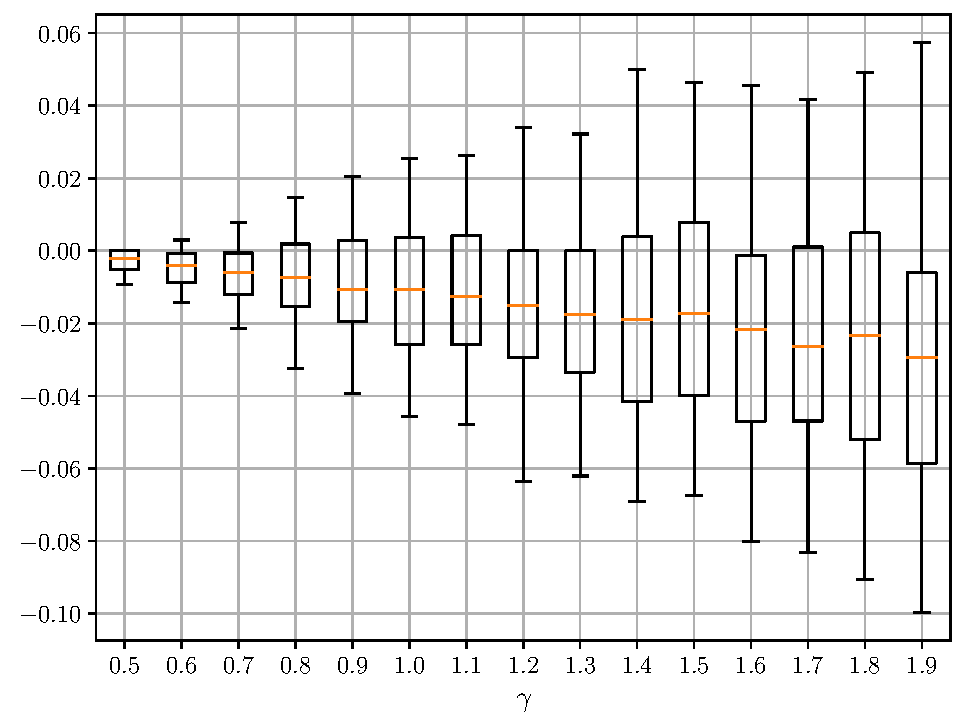
\includegraphics[width=0.8\linewidth]{images/part2/dir_est_05_20.pdf}
    \caption{Распределение относительной ошибки $\frac{\hat{k} - k}{\,k}$ в зависимости от параметра $\gamma$ для разработанного метода оценки (без учёта поправки на расщепления). Ящики показывают границы 25\% и 75\% квантилей, усики – 5\% и 95\% квантилей.}
    \label{dir_est_05_20}
\end{figure}

В таблице~\ref{tab-est-error} численно приведены средние абсолютные ошибки (в процентах) для нескольких выбранных значений $\gamma$. Можно заметить, что ошибка слегка возрастает с увеличением $\gamma$, но остаётся в пределах $5\%$ даже при $\gamma$ вплоть до $2.0$. Кроме того, при $\gamma < 0.5$ ошибка равна нулю (что соответствует режиму применимости парсимонии). Рост ошибки при больших $\gamma$ объясняется упомянутым систематическим эффектом недоучёта расщепления циклов в нашей аналитической модели. В реальных симуляциях не все циклы образуются только слиянием мелких компонентов: некоторая доля появляется из-за дробления крупных компонентов, что методически приводит к занижению оценённого $k$.

\begin{table}[!h]
  \caption{Средний модуль ошибки оценки $\hat{k}$ в процентах для разных значений $\gamma$.}
  \label{tab-est-error}
  \centering
  \begin{tabular}{|c|c||c|c|}
    \hline 
    $\gamma$ & $\;\text{Сред. ошибка}\;$ & $\gamma$ & $\;\text{Сред. ошибка}\;$ \\
    \hline
    $0.5$ & $0.3\%$ & $1.3$ & $2.78\%$ \\
    $0.6$ & $0.58\%$ & $1.4$ & $3.12\%$ \\
    $0.7$ & $0.86\%$ & $1.5$ & $3.14\%$ \\
    $0.8$ & $1.24\%$ & $1.6$ & $3.57\%$ \\
    $0.9$ & $1.59\%$ & $1.7$ & $3.76\%$ \\
    $1.0$ & $1.88\%$ & $1.8$ & $4.02\%$ \\
    $1.1$ & $2.10\%$ & $1.9$ & $4.49\%$ \\
    $1.2$ & $2.43\%$ & $2.0$ & $4.87\%$ \\
    \hline
  \end{tabular}
\end{table}

Как было отмечено, наш аналитический метод имеет тенденцию незначительно занижать оценки $k$ при больших $\gamma$. На рис.~\ref{dir_est_05_20} это проявляется в том, что медианные значения ошибки (серии внутри ящиков) лежат чуть ниже нуля при $\gamma > 1.0$, то есть $\hat{k}$ в среднем меньше настоящего $k$. Для компенсации этого эффекта можно ввести небольшую поправку. Эмпирически было найдено, что основная систематическая ошибка связана с недоучётом $d/n$ на величину порядка $0.1/\sqrt{n}$ при $\gamma \ge 0.5$, тогда как при $\gamma < 0.5$ ошибка отсутствует (что согласуется с тем, что при малом $\gamma$ расщепления действительно пренебрежимо редки). Поэтому можно скорректировать оценку, увеличивая $d$ на $\frac{0.1}{\sqrt{n}}$ (для $\gamma \ge 0.5$) перед вычислением отношения $r = d/b$. Эта поправка практически не влияет на случаи с большим $n$ или умеренным $\gamma$, но для крайних режимов слегка повышает оценку $k$. Результаты работы метода с учётом данной эмпирической правки показаны на рис.~\ref{dir_est_05_20_buffed}. Видно, что систематический сдвиг устранён: медианы ошибок теперь проходят практически по нулевой линии даже при максимальных $\gamma$. Таким образом, скорректированный метод выдаёт асимптотически несмещённые оценки $k$ во всём диапазоне параметров модели.

\begin{figure}[h!]
    \centering
    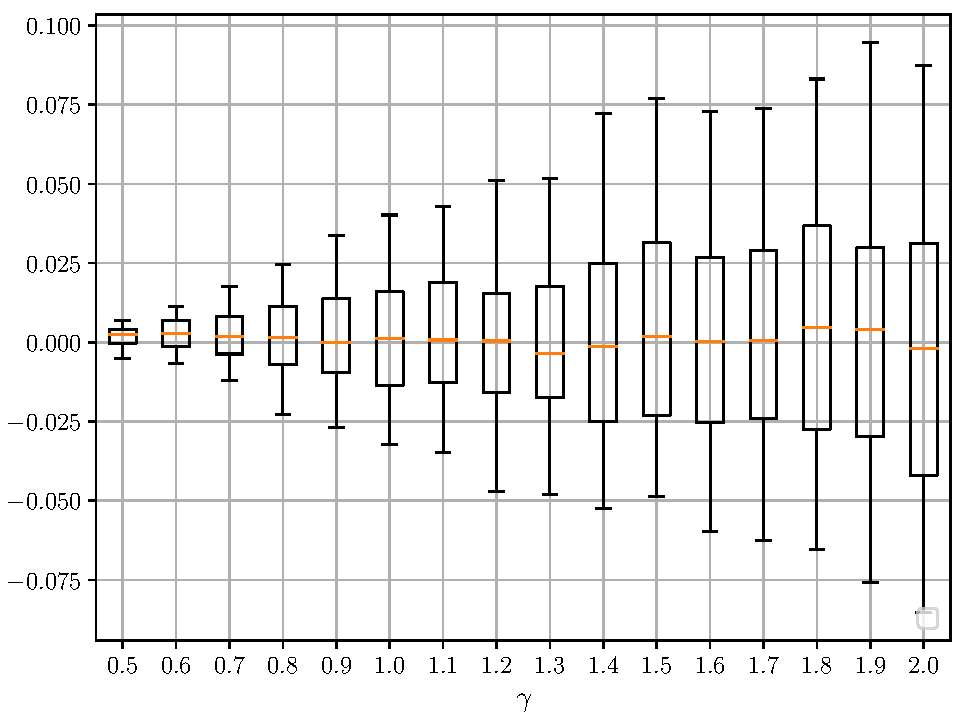
\includegraphics[width=0.8\linewidth]{images/part2/dir_est_05_20_buffed.pdf}
    \caption{Распределение относительной ошибки $\frac{\hat{k} - k}{\,k}$ после введения поправки на систематическое смещение (добавление $0.1/\sqrt{n}$ к $d/n$ при $\gamma \ge 0.5$). Сравните со случаем без поправки на рис.~\ref{dir_est_05_20}.}
    \label{dir_est_05_20_buffed}
\end{figure}

Таким образом, на синтетических данных подтверждается высокая точность предлагаемого метода оценки истинного эволюционного расстояния. В частности, метод корректно работает в той области параметров ($\gamma > 0.5$), где классический парсимонийный подход систематически недооценивает расстояние. На модельных примерах получено, что даже для существенно эволюционировавших структур (например, $\gamma = 2.0$, что соответствует $k \approx n$) новая оценка $\hat{k}$ отличается от реального значения $k$ менее чем на $5\%$ в среднем, тогда как парсимонийная оценка $d$ в таких случаях отличается на десятки процентов. 

Следует подчеркнуть, что описанные эксперименты проводились на \emph{модельных данных}, то есть на синтетических структурах, эволюционировавших строго в соответствии с предложенной случайной моделью (с заданными параметрами $\gamma$ и распределением хрупкостей). Это необходимо для валидации метода и соответствия условий его вывода. В следующей главе будет рассмотрено применение метода к реальным данным и оценено, насколько хорошо модель описывает реальные ситуации.

\section*{Выводы по главе 2}
\addcontentsline{toc}{section}{Выводы по главе~\ref{chap:random_graphs}}

В данной главе были разработаны и математически обоснованы методы анализа случайных графов, моделирующих геномные перестройки, и методы оценки истинного эволюционного расстояния между структурами. Основные результаты, полученные в этой главе, можно суммировать следующим образом:

\begin{enumerate}
    \item Разработан строгий комбинаторный подход к вычислению математического ожидания количества компонент заданного размера в графе несоответствия, основанный на биекции между сценариями объединения блоков и помеченными деревьями. Получены аналитические выражения для ожидаемого числа компонент произвольного размера.

    \item Выполнен асимптотический анализ поведения компонент в графе несоответствия при увеличении числа элементов $n$ и числа операций $k$. В частности, показано существование фазового перехода (при критическом значении $\gamma_c = 0.5$), после которого в системе возникает гигантская компонента, охватывающая существенную часть элементов структуры.

    \item Полученные формулы позволили построить новый статистический метод оценки истинного эволюционного расстояния между двумя структурами на основе наблюдаемых характеристик графа несоответствия (числа разрывов и парсимонийного расстояния). Метод учитывает нелинейную связь между числом разрывов и реальным числом перестроек, характерную для больших эволюционных расстояний.

    \item Проведена оценка точности предложенного метода на синтетических данных, моделирующих реалистичные сценарии эволюции геномных структур. Показано, что разработанный подход существенно превосходит парсимонийный метод в условиях большого числа перестроек (при $\gamma > 0.5$), давая ошибки оценки не более 5\%, тогда как классические подходы существенно недооценивают реальное число перестроек.

    \item Вспомогательные математические результаты (например, вычисления многомерных интегралов и использование кодов Прюфера для подсчёта вероятностей сценариев) имеют самостоятельное значение и могут быть использованы при решении других комбинаторных задач в области стохастического анализа графовых моделей.

\end{enumerate}

Таким образом, результаты второй главы обеспечивают строгую математическую основу для количественной оценки эволюционных перестроек, подготавливая почву для применения и валидации этих методов на реальных биологических данных, чему посвящены последующие главы.
